\documentclass[conference]{IEEEtran}
% Some Computer Society conferences also require the compsoc mode option,
% but others use the standard conference format.
%
% If IEEEtran.cls has not been installed into the LaTeX system files,
% manually specify the path to it like:
% \documentclass[conference]{../sty/IEEEtran}





% Some very useful LaTeX packages include:
% (uncomment the ones you want to load)


% *** MISC UTILITY PACKAGES ***
%
%\usepackage{ifpdf}
% Heiko Oberdiek's ifpdf.sty is very useful if you need conditional
% compilation based on whether the output is pdf or dvi.
% usage:
% \ifpdf
%   % pdf code
% \else
%   % dvi code
% \fi
% The latest version of ifpdf.sty can be obtained from:
% http://www.ctan.org/pkg/ifpdf
% Also, note that IEEEtran.cls V1.7 and later provides a builtin
% \ifCLASSINFOpdf conditional that works the same way.
% When switching from latex to pdflatex and vice-versa, the compiler may
% have to be run twice to clear warning/error messages.






% *** CITATION PACKAGES ***
%
%\usepackage{cite}
% cite.sty was written by Donald Arseneau
% V1.6 and later of IEEEtran pre-defines the format of the cite.sty package
% \cite{} output to follow that of the IEEE. Loading the cite package will
% result in citation numbers being automatically sorted and properly
% "compressed/ranged". e.g., [1], [9], [2], [7], [5], [6] without using
% cite.sty will become [1], [2], [5]--[7], [9] using cite.sty. cite.sty's
% \cite will automatically add leading space, if needed. Use cite.sty's
% noadjust option (cite.sty V3.8 and later) if you want to turn this off
% such as if a citation ever needs to be enclosed in parenthesis.
% cite.sty is already installed on most LaTeX systems. Be sure and use
% version 5.0 (2009-03-20) and later if using hyperref.sty.
% The latest version can be obtained at:
% http://www.ctan.org/pkg/cite
% The documentation is contained in the cite.sty file itself.






% *** GRAPHICS RELATED PACKAGES ***
%
\ifCLASSINFOpdf
   \usepackage[pdftex]{graphicx}
  % declare the path(s) where your graphic files are
  % \graphicspath{{../pdf/}{../jpeg/}}
  % and their extensions so you won't have to specify these with
  % every instance of \includegraphics
  % \DeclareGraphicsExtensions{.pdf,.jpeg,.png}
\else
  % or other class option (dvipsone, dvipdf, if not using dvips). graphicx
  % will default to the driver specified in the system graphics.cfg if no
  % driver is specified.
   \usepackage[dvips]{graphicx}
  % declare the path(s) where your graphic files are
  % \graphicspath{{../eps/}}
  % and their extensions so you won't have to specify these with
  % every instance of \includegraphics
  % \DeclareGraphicsExtensions{.eps}
\fi
% graphicx was written by David Carlisle and Sebastian Rahtz. It is
% required if you want graphics, photos, etc. graphicx.sty is already
% installed on most LaTeX systems. The latest version and documentation
% can be obtained at: 
% http://www.ctan.org/pkg/graphicx
% Another good source of documentation is "Using Imported Graphics in
% LaTeX2e" by Keith Reckdahl which can be found at:
% http://www.ctan.org/pkg/epslatex
%
% latex, and pdflatex in dvi mode, support graphics in encapsulated
% postscript (.eps) format. pdflatex in pdf mode supports graphics
% in .pdf, .jpeg, .png and .mps (metapost) formats. Users should ensure
% that all non-photo figures use a vector format (.eps, .pdf, .mps) and
% not a bitmapped formats (.jpeg, .png). The IEEE frowns on bitmapped formats
% which can result in "jaggedy"/blurry rendering of lines and letters as
% well as large increases in file sizes.
%
% You can find documentation about the pdfTeX application at:
% http://www.tug.org/applications/pdftex





% *** MATH PACKAGES ***
%
%\usepackage{amsmath}
% A popular package from the American Mathematical Society that provides
% many useful and powerful commands for dealing with mathematics.
%
% Note that the amsmath package sets \interdisplaylinepenalty to 10000
% thus preventing page breaks from occurring within multiline equations. Use:
%\interdisplaylinepenalty=2500
% after loading amsmath to restore such page breaks as IEEEtran.cls normally
% does. amsmath.sty is already installed on most LaTeX systems. The latest
% version and documentation can be obtained at:
% http://www.ctan.org/pkg/amsmath





% *** SPECIALIZED LIST PACKAGES ***
%
%\usepackage{algorithmic}
% algorithmic.sty was written by Peter Williams and Rogerio Brito.
% This package provides an algorithmic environment fo describing algorithms.
% You can use the algorithmic environment in-text or within a figure
% environment to provide for a floating algorithm. Do NOT use the algorithm
% floating environment provided by algorithm.sty (by the same authors) or
% algorithm2e.sty (by Christophe Fiorio) as the IEEE does not use dedicated
% algorithm float types and packages that provide these will not provide
% correct IEEE style captions. The latest version and documentation of
% algorithmic.sty can be obtained at:
% http://www.ctan.org/pkg/algorithms
% Also of interest may be the (relatively newer and more customizable)
% algorithmicx.sty package by Szasz Janos:
% http://www.ctan.org/pkg/algorithmicx




% *** ALIGNMENT PACKAGES ***
\usepackage{booktabs}
\usepackage{array}
% Frank Mittelbach's and David Carlisle's array.sty patches and improves
% the standard LaTeX2e array and tabular environments to provide better
% appearance and additional user controls. As the default LaTeX2e table
% generation code is lacking to the point of almost being broken with
% respect to the quality of the end results, all users are strongly
% advised to use an enhanced (at the very least that provided by array.sty)
% set of table tools. array.sty is already installed on most systems. The
% latest version and documentation can be obtained at:
% http://www.ctan.org/pkg/array





% *** SUBFIGURE PACKAGES ***
%\ifCLASSOPTIONcompsoc
%  \usepackage[caption=false,font=normalsize,labelfont=sf,textfont=sf]{subfig}
%\else
%  \usepackage[caption=false,font=footnotesize]{subfig}
%\fi
% subfig.sty, written by Steven Douglas Cochran, is the modern replacement
% for subfigure.sty, the latter of which is no longer maintained and is
% incompatible with some LaTeX packages including fixltx2e. However,
% subfig.sty requires and automatically loads Axel Sommerfeldt's caption.sty
% which will override IEEEtran.cls' handling of captions and this will result
% in non-IEEE style figure/table captions. To prevent this problem, be sure
% and invoke subfig.sty's "caption=false" package option (available since
% subfig.sty version 1.3, 2005/06/28) as this is will preserve IEEEtran.cls
% handling of captions.
% Note that the Computer Society format requires a larger sans serif font
% than the serif footnote size font used in traditional IEEE formatting
% and thus the need to invoke different subfig.sty package options depending
% on whether compsoc mode has been enabled.
%
% The latest version and documentation of subfig.sty can be obtained at:
% http://www.ctan.org/pkg/subfig




% *** FLOAT PACKAGES ***
%
%\usepackage{fixltx2e}
% fixltx2e, the successor to the earlier fix2col.sty, was written by
% Frank Mittelbach and David Carlisle. This package corrects a few problems
% in the LaTeX2e kernel, the most notable of which is that in current
% LaTeX2e releases, the ordering of single and double column floats is not
% guaranteed to be preserved. Thus, an unpatched LaTeX2e can allow a
% single column figure to be placed prior to an earlier double column
% figure.
% Be aware that LaTeX2e kernels dated 2015 and later have fixltx2e.sty's
% corrections already built into the system in which case a warning will
% be issued if an attempt is made to load fixltx2e.sty as it is no longer
% needed.
% The latest version and documentation can be found at:
% http://www.ctan.org/pkg/fixltx2e


%\usepackage{stfloats}
% stfloats.sty was written by Sigitas Tolusis. This package gives LaTeX2e
% the ability to do double column floats at the bottom of the page as well
% as the top. (e.g., "\begin{figure*}[!b]" is not normally possible in
% LaTeX2e). It also provides a command:
%\fnbelowfloat
% to enable the placement of footnotes below bottom floats (the standard
% LaTeX2e kernel puts them above bottom floats). This is an invasive package
% which rewrites many portions of the LaTeX2e float routines. It may not work
% with other packages that modify the LaTeX2e float routines. The latest
% version and documentation can be obtained at:
% http://www.ctan.org/pkg/stfloats
% Do not use the stfloats baselinefloat ability as the IEEE does not allow
% \baselineskip to stretch. Authors submitting work to the IEEE should note
% that the IEEE rarely uses double column equations and that authors should try
% to avoid such use. Do not be tempted to use the cuted.sty or midfloat.sty
% packages (also by Sigitas Tolusis) as the IEEE does not format its papers in
% such ways.
% Do not attempt to use stfloats with fixltx2e as they are incompatible.
% Instead, use Morten Hogholm'a dblfloatfix which combines the features
% of both fixltx2e and stfloats:
%
% \usepackage{dblfloatfix}
% The latest version can be found at:
% http://www.ctan.org/pkg/dblfloatfix




% *** PDF, URL AND HYPERLINK PACKAGES ***
%
\usepackage{url}
% url.sty was written by Donald Arseneau. It provides better support for
% handling and breaking URLs. url.sty is already installed on most LaTeX
% systems. The latest version and documentation can be obtained at:
% http://www.ctan.org/pkg/url
% Basically, \url{my_url_here}.




% *** Do not adjust lengths that control margins, column widths, etc. ***
% *** Do not use packages that alter fonts (such as pslatex).         ***
% There should be no need to do such things with IEEEtran.cls V1.6 and later.
% (Unless specifically asked to do so by the journal or conference you plan
% to submit to, of course. )
\usepackage{filecontents}
\usepackage[noadjust]{cite}

\begin{filecontents*}{bibi.bib}
	@misc{NoC,
		title = {Applying the Benefits of Network on a Chip Architecture to FPGA System Design},
		author={Altera Corporation},
		date = {April, 2011},
		OPTurl = {https://www.altera.com/en\_US/pdfs/literature/wp/wp-01149-noc-qsys.pdf},
	}
	@book{appel2004modern,
		title={Modern compiler implementation in C},
		author={Appel, Andrew W},
		year={2004},
		publisher={Cambridge university press}
	}
\end{filecontents*}


% correct bad hyphenation here
\hyphenation{op-tical net-works semi-conduc-tor}


\begin{document}
%
% paper title
% Titles are generally capitalized except for words such as a, an, and, as,
% at, but, by, for, in, nor, of, on, or, the, to and up, which are usually
% not capitalized unless they are the first or last word of the title.
% Linebreaks \\ can be used within to get better formatting as desired.
% Do not put math or special symbols in the title.
\title{IL2212 Embedded Software\\Lab 2 Report\\Session: Friday Morning}


% author names and affiliations
% use a multiple column layout for up to three different
% affiliations
\author{\IEEEauthorblockN{Yuefeng Wu}
\IEEEauthorblockA{Embedded Systems\\
EIT Digital Master School\\
Personal Number: 921116-6039\\
Email: yuefeng@kth.se}
\and
\IEEEauthorblockN{Renzhi Xing}
\IEEEauthorblockA{Embedded Systems\\
KTH, Royal Institute of Technology\\
Personal Number: 931011-2025\\
Email: renzhi@kth.se}
}

% conference papers do not typically use \thanks and this command
% is locked out in conference mode. If really needed, such as for
% the acknowledgment of grants, issue a \IEEEoverridecommandlockouts
% after \documentclass

% for over three affiliations, or if they all won't fit within the width
% of the page, use this alternative format:
% 
%\author{\IEEEauthorblockN{Michael Shell\IEEEauthorrefmark{1},
%Homer Simpson\IEEEauthorrefmark{2},
%James Kirk\IEEEauthorrefmark{3}, 
%Montgomery Scott\IEEEauthorrefmark{3} and
%Eldon Tyrell\IEEEauthorrefmark{4}}
%\IEEEauthorblockA{\IEEEauthorrefmark{1}School of Electrical and Computer Engineering\\
%Georgia Institute of Technology,
%Atlanta, Georgia 30332--0250\\ Email: see http://www.michaelshell.org/contact.html}
%\IEEEauthorblockA{\IEEEauthorrefmark{2}Twentieth Century Fox, Springfield, USA\\
%Email: homer@thesimpsons.com}
%\IEEEauthorblockA{\IEEEauthorrefmark{3}Starfleet Academy, San Francisco, California 96678-2391\\
%Telephone: (800) 555--1212, Fax: (888) 555--1212}
%\IEEEauthorblockA{\IEEEauthorrefmark{4}Tyrell Inc., 123 Replicant Street, Los Angeles, California 90210--4321}}




% use for special paper notices
%\IEEEspecialpapernotice{(Invited Paper)}




% make the title area
\maketitle

% As a general rule, do not put math, special symbols or citations
% in the abstract
\begin{abstract}
This report is a laboratory record of Lab 2 in IL2212 Embedded Software VT2016. In this report, we will present the implementation procedures of required functions: loading RGB images to on-chip memory, turning the images into gray-scale format, resizing the converted images, performing edge detection algorithm on the resized images and finally saving ASCII images into shared on-chip memory. Additionally, we will give a relatively detailed analysis of the application's throughput and document optimizations. 
\end{abstract}

% no keywords




% For peer review papers, you can put extra information on the cover
% page as needed:
% \ifCLASSOPTIONpeerreview
% \begin{center} \bfseries EDICS Category: 3-BBND \end{center}
% \fi
%
% For peerreview papers, this IEEEtran command inserts a page break and
% creates the second title. It will be ignored for other modes.
\IEEEpeerreviewmaketitle



\section{Introduction}
In this laboratory, we are required to implement a image processing algorithm on three systems based on different hardware configurations. On the Bare-Metal single core and $\mu$/C-OS II single core systems, we implemented required algorithm and verified the results, which consolidated our fundamental knowledge of the NIOS II and $\mu$/C-OS II. And additionally we are required to transplant our code onto a multiprocessor system. During the transplantation procedure, we can get a deep insight of multiprocessing, hardware architecture and code optimization. 

\section{Single Processor Application Description}
In the skeleton of the application, a macro was predefined to distinguish debug mode and performance mode. We implemented the debug-mode functions in single processor platforms(both on Bare-Metal and $\mu$C-OS II) and the performance mode code on multiprocessor platform.\\
\subsection{Loading images to shared memory}
This function is given by the skeleton. We used the similar coding theme in other functions---using pointers instead of arrays to access and process matrix.\\
\indent
On the other hand, according to the qsys file and the auto-compilation script, the default code space of cpu\_0 is SRAM, which means that the default storage location is SRAM. The images are stored in the \emph{image.h} located in SRAM. And the function teaches us to use address to access the shared on-chip memory.\\
\indent
However, since the access speed of SRAM is significantly slower than the on-chip 
\subsection{Converting RGB images into grayscale}
The computation formula of the conversion is:
\begin{center}
	\emph{Y = 0.3125 $\times$ R + 0.5625 $\times$ G + 0.125 $\times$ B}
\end{center}
After some experiment, we found that this function consumed a relatively larger amount of storage space and execution time. We currently have made two main optimizations.
\begin{itemize}
	\item{\textbf{Reuse of shared on-chip memory}}\\
	According to the memory management strategy, the two dimension array is stored as a line of data blocks. And the gray scale algorithm is to combine three 8 bytes data into one. So we can reuse the RGB image's part of on-chip memory. We drew a simple graph to demonstrate the reusing procedure.
	\begin{figure}
		\centering
		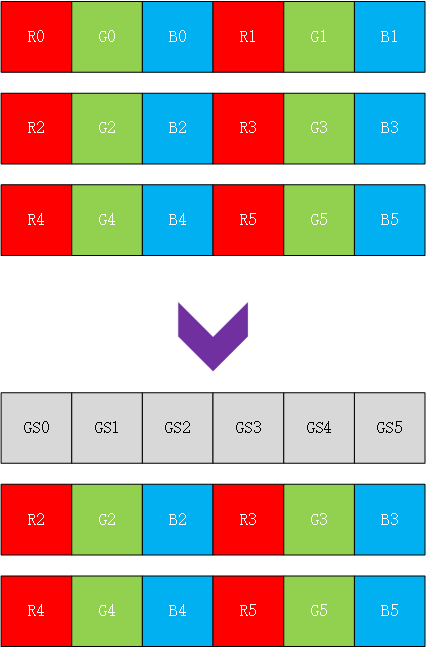
\includegraphics[scale=0.5]{reuse.png}
		\caption{On-chip memory reuse strategy for gray scale}
		\label{fg:reuse}
	\end{figure}
	\item{\textbf{Avoiding float computation}}\\
	After several executions, we found that the float computation required much more CPU time compared to integer. \\
	To avoid float computation, we firstly made the RGB value multiplied by 5, 9 and 2 respectively and summed them up. Then we divide the sum with 16. All the multiplications and divisions were all replaced by left-shifting and right-shifting.\\
	To indicate the effect the optimization, we built a table for the comparison.
\end{itemize}
\begin{table}
	\centering
	\caption{Comparison between integer and float computation}
	\label{tab:Compare}
	\begin{tabular}{ccc}
		\toprule
		Image size& Float(sec)& Integer(sec)\\
		\midrule
		$24\times24$& 0.788& 0.269\\
		$32\times22$& 1.069& 0.241\\
		$32\times22$& 1.448& 0.292\\
		$40\times28$& 1.898& 0.316\\
		$40\times40$& 2.251& 0.412\\
		\bottomrule
	\end{tabular}
\end{table}
\subsection{Resizing the grayscale images}
This function can also reuse the on-chip memory. We used this feature for optimization and drew a simple graph to demonstrate the reuse.
\begin{figure}
	\centering
	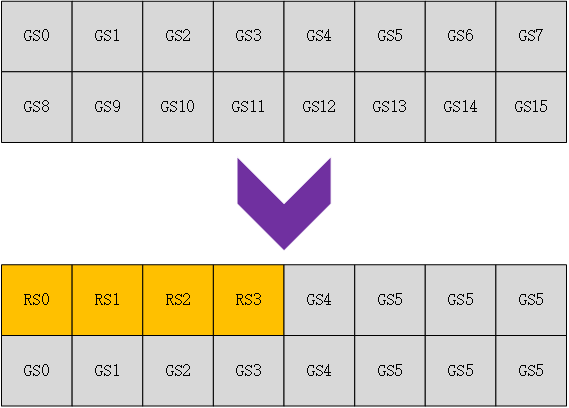
\includegraphics[scale=0.5]{resize.png}
	\caption{On-chip memory reuse strategy for resizing}
	\label{fg:resize}
\end{figure}
\subsection{Edge detection with Sobel core}
Firstly, we made an approximation on the formula of the gradient magnitude. We replaced
\begin{center}
	$G = \sqrt{{G_x}^2 + {G_y}^2}$
\end{center}
with
\begin{center}
	$G = |G_x| + |G_y|$
\end{center}
to reduce the computational work. After we made this approximation, we also removed redundant absolute value computation since calling for \emph{abs()} function would also increase execution time.\\
\indent
We divided the image matrix into 9 parts, which is described in the figure. In some cases, $G_x$ or $G_y$ will always be positive or negative, then we removed the calling. For example, at the point $(0,0)$, the $G_x$ and $G_y$ will always be positive.
\begin{figure}
	\centering
	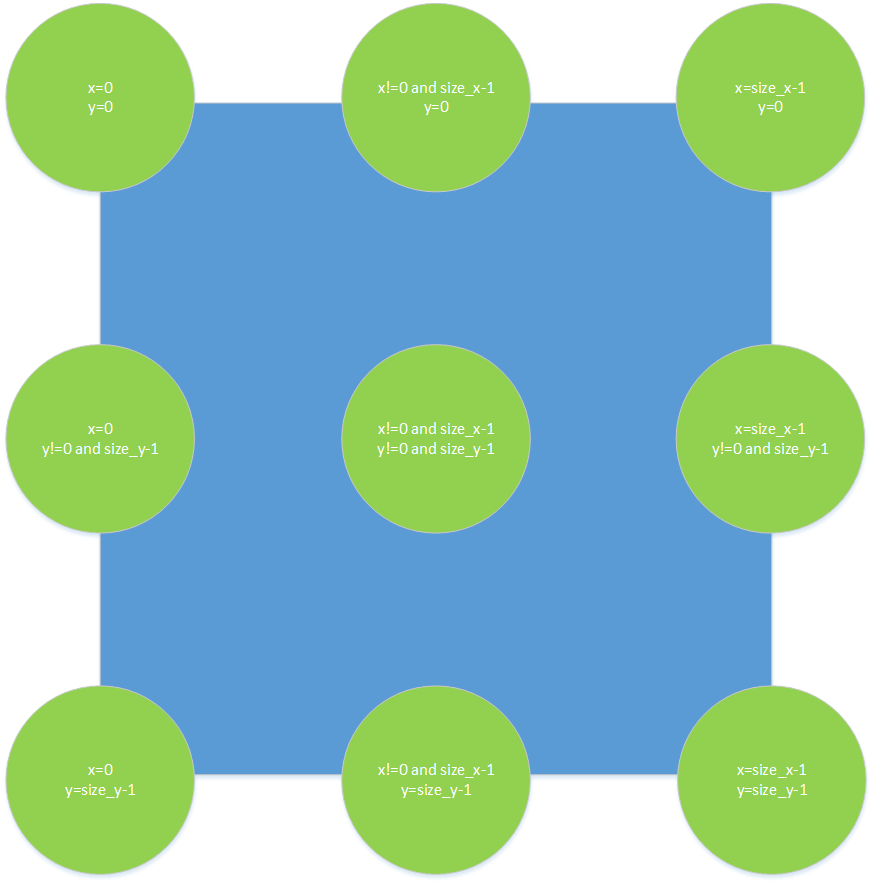
\includegraphics[scale=0.3]{part.png}
	\caption{Parts of the image matrix}
	\label{fg:part}
\end{figure}
\section{Multi-processor Application Description}
\subsection{Processor Assignment}
The final version of application architecture is different from the firstly proposed structure. In this version, we make cpu\_0 responsible for loading image from SRAM to shared on-chip memory and storing ASCII image to SRAM. And cpu\_1 to cpu\_4 are designed to grayscale, resize representative part of the RGB image in shared on-chip memory. Unfortunately, due to the synchronization issue, we eventually assigned the computation of edge detection and ASCII image only to cpu\_1. However, this compromise has slight influence on the throughput, which will be talked in detail in the section of \emph{Software Pipeline}.
\begin{figure*}
	\centering
	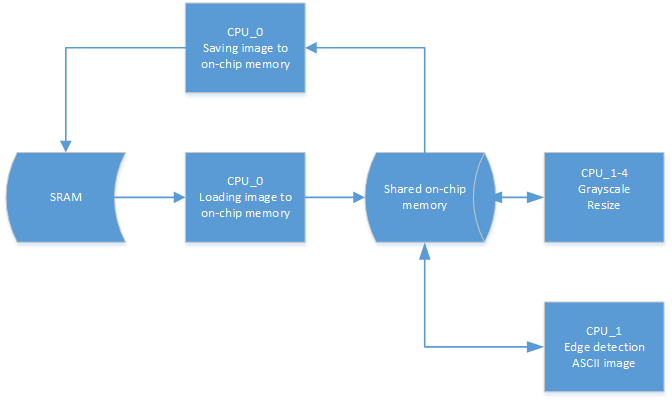
\includegraphics[scale=1]{mparch.png}
	\caption{Multiprocessor application architecture}
	\label{fg:mpapp}
\end{figure*}
\subsection{Shared Memory Mapping}
In the predefined multiprocessor system, a 8 KByte shared on-chip memory builds a bridge for the communications between five cores. Since it is a part of on-chip memory, its speed of access is much faster than SRAM.\\
\indent
We divided the shared memory into five parts--RGB image, grayscale image, resized image, semaphores and image information. We built a table to indicate the mapping strategy more directly.
\begin{table}
	\centering
	\caption{Shared on-chip memory mapping}
	\label{tab:Mapping}
	\begin{tabular}{cccc}
		\toprule
		Content&Start(dec)&End(dec)&Size(byte)\\
		\midrule
		RGB image&0&4095&4096\\
		Grayscale image&4096&5119&1024\\
		Resized image&5120&5375&256\\
		ASCII image&6144&6400&256\\
		Semaphore 1-8 &7168&7207&32\\
		Image information&8184&8186&3\\
		\bottomrule
	\end{tabular}
\end{table}
\subsection{Synchronization}
As mentioned above, we used some part of shared on-chip memory to implement semaphores.\\
\indent
Semaphore is a good mechanism to synchronize threads or cores for accessing the shared resources. In our application, we used semaphores to avoid simultaneous reading and writing to the same part of memory from different cores. For example, if cpu\_1 is grayscaling the image in the shared memory and cpu\_0 is loading a new image to shared memory at the same time, there will be a inevitable collision that make the generated grayscale image incorrect.\\
\indent
In our application, we designed two kinds of semaphores--\emph{key semaphore and feedback semaphore}.\\
\indent
\emph{Key semaphore} is the key to start the next procedure. After one precedent procedure is finished and the data required by following procedure is prepared, the precedent procedure sends a key semaphore to the following one to start it. For example, \emph{SEMAPHORE\_3} in our application is sent by grayscale procedure to resizing after the loaded image is grayscaled. The key semaphores need to be initialized with 0 in application initialization.\\
\indent
\emph{Feedback semaphore} is the feedback from following procedure to precedent one, which entitle the precedent procedure to write data to allocated memory. For example, \emph{SEMAPHORE\_8} is sent by Sobel value computation procedure to resizing to inform it to continue resizing one new image. The feedback semaphores need to be initialized with 1, otherwise the application won't execute properly.\\
\indent
We drew a interference graph to demonstrate the synchronization mechanism.
\begin{figure}
	\centering
	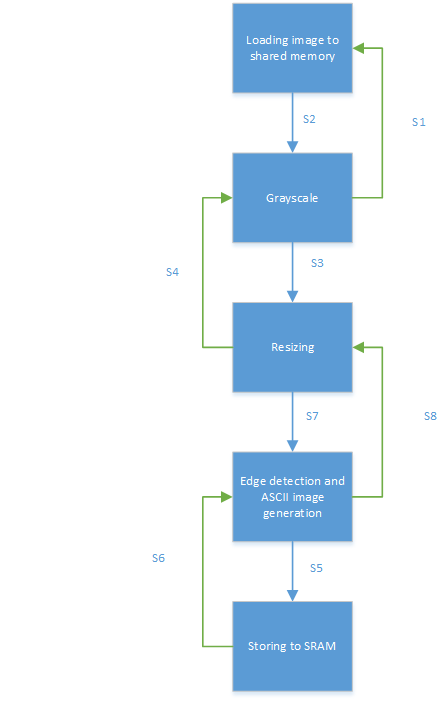
\includegraphics[scale=0.8]{sync.png}
	\caption{Semaphore interference graph. Blue for key semaphores, green for feedback semaphores.}
	\label{fg:sync}
\end{figure}
\subsection{Software Pipeline}
The most time-consuming procedure in our application is loading RGB image to shared memory, since the amount of data is relatively larger and access speed of SRAM is slower than on-chip memory. After optimizations, we finally reduced the execution time of loading image to about 870 $\mu$s, which still constitute most part of total execution time. To reduce execution time, we built a software pipeline to assign other jobs to cpu\_1-cpu\_4. We also drew a graph to demonstrate the pipeline. In the size-based optimized code, we used dual-core system, we also drew the pipeline graph.\\
\begin{figure*}
	\centering
	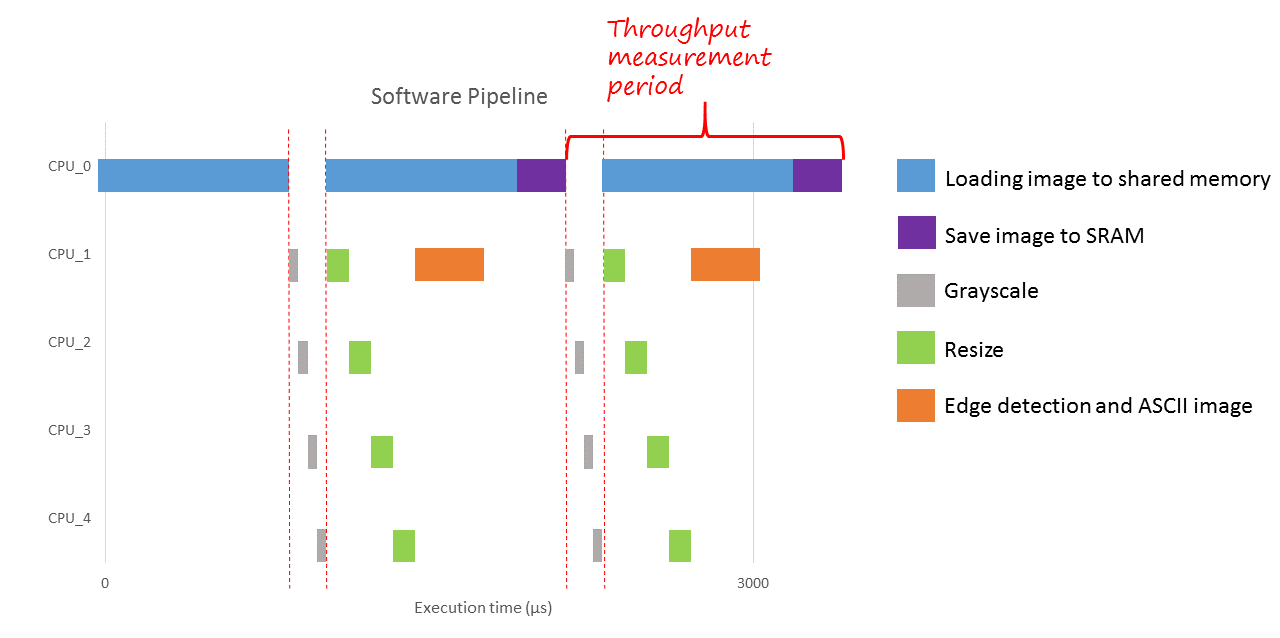
\includegraphics[scale=0.55]{pipeline.png}
	\caption{Software pipeline of the penta-core system}
	\label{fg:pipeline}
\end{figure*}
\begin{figure*}
	\centering
	\label{fig:Dualcore}
	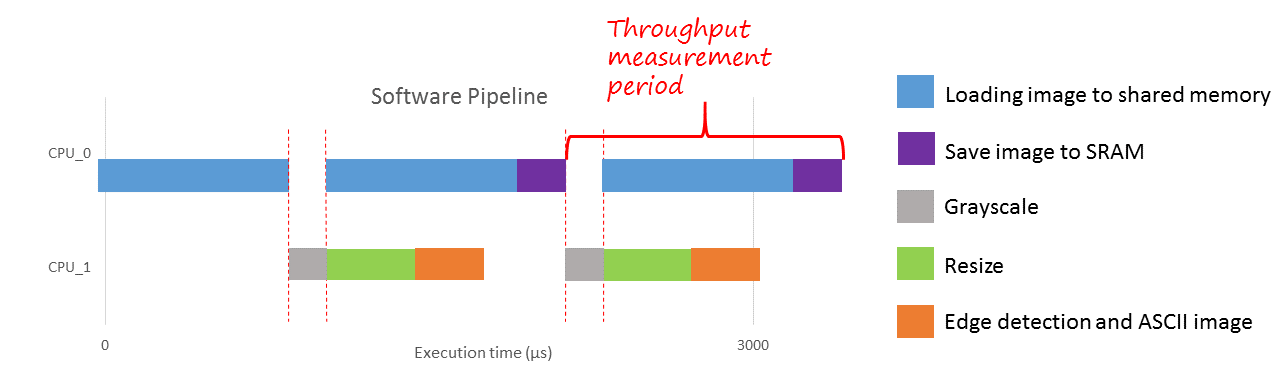
\includegraphics[scale=0.55]{dualcore.png}
	\caption{Software pipeline of the dual-core system}
\end{figure*}
\indent
As the graph indicated, the cpu\_1-cpu\_4 will do resizing, compute Sobel value and generate ASCII image while cpu\_0 is loading image to on-chip memory. As long as the total execution time of multiple procedures of cpu\_1-cpu\_4 doesn't exceed the image-loading time of cpu\_0, there will be nearly no influence on the final execution time. This is the reason why we eventually assign the Sobel and ASCII image computation only to cpu\_1 to avoid synchronization issues.
\section{Final Throughput}
We measured the final throughput by calculating the average execution time of three $32\times32$ images and get its multiplicative inverse. Here is the throughput table. All the code is running in performance mode. And another thing to be mentioned is that the throughputs of single-core applications ($\mu$/C-OS II and bare metal) is based on unoptimized codes.
\begin{table*}
	\centering
	\caption{Final throughput}
	\label{tab:Throughput}
	\begin{tabular}{l|cccc}
		\toprule
		&Single core (RTOS)&Single Core (Bare-Metal)&Multicore (5 cores)&Multicore (2 cores)\\
		\midrule
		Throughput ($s^{-1}$)&\textbf{103}&\textbf{197}&\textbf{1114}&\textbf{1114}\\	
		SRAM (Byte)&146484&42836&45116&44556\\
		OnChip CPU 1 (Byte)&-&-&2420&2360\\
		OnChip CPU 2 (Byte)&-&-&1696&-\\
		OnChip CPU 3 (Byte)&-&-&1696&-\\
		OnChip CPU 4 (Byte)&-&-&1664&-\\
		Shared OnChip (Byte)&3075&3075&5667&5385\\
		Total Memory (Byte)&149559&45911&58517&52301\\
		\bottomrule
	\end{tabular}
\end{table*}

\section{Optimizations}
In this section, we only talk about three significant optimizations that cast a huge influence on the total execution time.
\subsection{Utilization of 32bit Data Bus}
This optimization significantly reduces the execution time of loading image to shared on-chip memory by more than 2000 $\mu$s. The given \emph{sram2sm\_p3()} function transmits the image pixels by 8 bit data every time. However, the data bus of the system is 32bit. We defined two integer (32bit) pointers which point to the data in SRAM and shared on-chip memory respectively and transmitted data between the pointers. This optimization cuts down the execution time by 4 times since the iteration of transmission is reduces.
\subsection{Replacing Multiplication and Division}
This optimization replaces time-consuming multiplication and division with shifting. CPUs can perform shifting much faster than multiplication and division. Since the Sobel computation contains a lot of multiplication, this optimization has an apparent influence on the final execution time.
\subsection{Macros}
We defined a lot of macros to reduce code size and debug conveniently. On the other hand, the well-defined macros can also make the source code more readable.
\section{Discussion and Analysis}
In this section, we will give some discussion and analysis on our final result. The points discussed are questions emerged while developing the applications.
\subsection{Dual-core V.S. Penta-core}
From the \emph{Table III} we can see that the final through puts of dual-core and penta-core platforms are the same (actually, the dual-core is a little bit faster if we check the clock circles). The phenomenon can be explained by the access limitation of shared on-chip memory. According to the \emph{Network on Chip} architecture, the data need to be transmitted in "packages" and the slave (shared on-chip memory) can only accept one package at one time\cite{NoC}. So even if we hope to let the cpu\_1 to cpu\_4 grayscale the image in shared on-chip memory simultaneously, they still have to queue to get own turn to read and write the shared memory. So they final throughputs are nearly the same.
\subsection{Different Execution Time Between cpu\_0 and cpu\_1-4}
Firstly, we built a table for the execution time on the single core (cpu\_0) of every step. From the table we can see that grayscaling, resizing and edge detecting a 32$\times$32 image need a much longer time than loading it from SRAM to shared on-chip memory.\\ 
\begin{table}[h]
	\centering
	\caption{The execution time of procedures on cpu\_0}
	\label{tab:SinglecoreExeTime}
	\begin{tabular}{l|c}
		\toprule
		Section&Execution time ($\mu$sec)\\
		\midrule
		Loading from SRAM&3206\\
		Grayscale&4218\\
		Resizing&1225\\
		Sobel&2733\\
		\midrule
		Total&11382\\
		\bottomrule
	\end{tabular}
\end{table}
\indent
However, since the default code space for cpu\_1-4 is on-chip memory while cpu\_0's is SRAM and SRAM performs much slower than on-chip memory, writing and reading a temporary variable can be significantly faster on cpu\_1-4. So the procedures can consume less execution time on cpu\_1-4 than on cpu\_0. 
\subsection{Further Optimization of Loading Image from SRAM}
We firstly got a throughput of 954 $s^{-1}$ and the execution time of loading a image from SRAM was about 950 $\mu$s. We finally decrease the execution time to around 870 $\mu$s by eliminating the function call of \emph{IOWR\_32DIRECT()} and using 32-bit data pointers to transmit data directly.\\
\indent
Elimination of function calls can reduce the time consumption because the calls need extra register and memory operations according to the calling conventions of compilers. To process a function call, an update of stack frames is needed, which consumes some time\cite{appel2004modern}.
% An example of a floating figure using the graphicx package.
% Note that \label must occur AFTER (or within) \caption.
% For figures, \caption should occur after the \includegraphics.
% Note that IEEEtran v1.7 and later has special internal code that
% is designed to preserve the operation of \label within \caption
% even when the captionsoff option is in effect. However, because
% of issues like this, it may be the safest practice to put all your
% \label just after \caption rather than within \caption{}.
%
% Reminder: the "draftcls" or "draftclsnofoot", not "draft", class
% option should be used if it is desired that the figures are to be
% displayed while in draft mode.
%
%\begin{figure}[!t]
%\centering
%\includegraphics[width=2.5in]{myfigure}
% where an .eps filename suffix will be assumed under latex, 
% and a .pdf suffix will be assumed for pdflatex; or what has been declared
% via \DeclareGraphicsExtensions.
%\caption{Simulation results for the network.}
%\label{fig_sim}
%\end{figure}

% Note that the IEEE typically puts floats only at the top, even when this
% results in a large percentage of a column being occupied by floats.


% An example of a double column floating figure using two subfigures.
% (The subfig.sty package must be loaded for this to work.)
% The subfigure \label commands are set within each subfloat command,
% and the \label for the overall figure must come after \caption.
% \hfil is used as a separator to get equal spacing.
% Watch out that the combined width of all the subfigures on a 
% line do not exceed the text width or a line break will occur.
%
%\begin{figure*}[!t]
%\centering
%\subfloat[Case I]{\includegraphics[width=2.5in]{box}%
%\label{fig_first_case}}
%\hfil
%\subfloat[Case II]{\includegraphics[width=2.5in]{box}%
%\label{fig_second_case}}
%\caption{Simulation results for the network.}
%\label{fig_sim}
%\end{figure*}
%
% Note that often IEEE papers with subfigures do not employ subfigure
% captions (using the optional argument to \subfloat[]), but instead will
% reference/describe all of them (a), (b), etc., within the main caption.
% Be aware that for subfig.sty to generate the (a), (b), etc., subfigure
% labels, the optional argument to \subfloat must be present. If a
% subcaption is not desired, just leave its contents blank,
% e.g., \subfloat[].


% An example of a floating table. Note that, for IEEE style tables, the
% \caption command should come BEFORE the table and, given that table
% captions serve much like titles, are usually capitalized except for words
% such as a, an, and, as, at, but, by, for, in, nor, of, on, or, the, to
% and up, which are usually not capitalized unless they are the first or
% last word of the caption. Table text will default to \footnotesize as
% the IEEE normally uses this smaller font for tables.
% The \label must come after \caption as always.
%
%\begin{table}[!t]
%% increase table row spacing, adjust to taste
%\renewcommand{\arraystretch}{1.3}
% if using array.sty, it might be a good idea to tweak the value of
% \extrarowheight as needed to properly center the text within the cells
%\caption{An Example of a Table}
%\label{table_example}
%\centering
%% Some packages, such as MDW tools, offer better commands for making tables
%% than the plain LaTeX2e tabular which is used here.
%\begin{tabular}{|c||c|}
%\hline
%One & Two\\
%\hline
%Three & Four\\
%\hline
%\end{tabular}
%\end{table}


% Note that the IEEE does not put floats in the very first column
% - or typically anywhere on the first page for that matter. Also,
% in-text middle ("here") positioning is typically not used, but it
% is allowed and encouraged for Computer Society conferences (but
% not Computer Society journals). Most IEEE journals/conferences use
% top floats exclusively. 
% Note that, LaTeX2e, unlike IEEE journals/conferences, places
% footnotes above bottom floats. This can be corrected via the
% \fnbelowfloat command of the stfloats package.


%\newpage
%\begin{figure*}
%	\centering
%	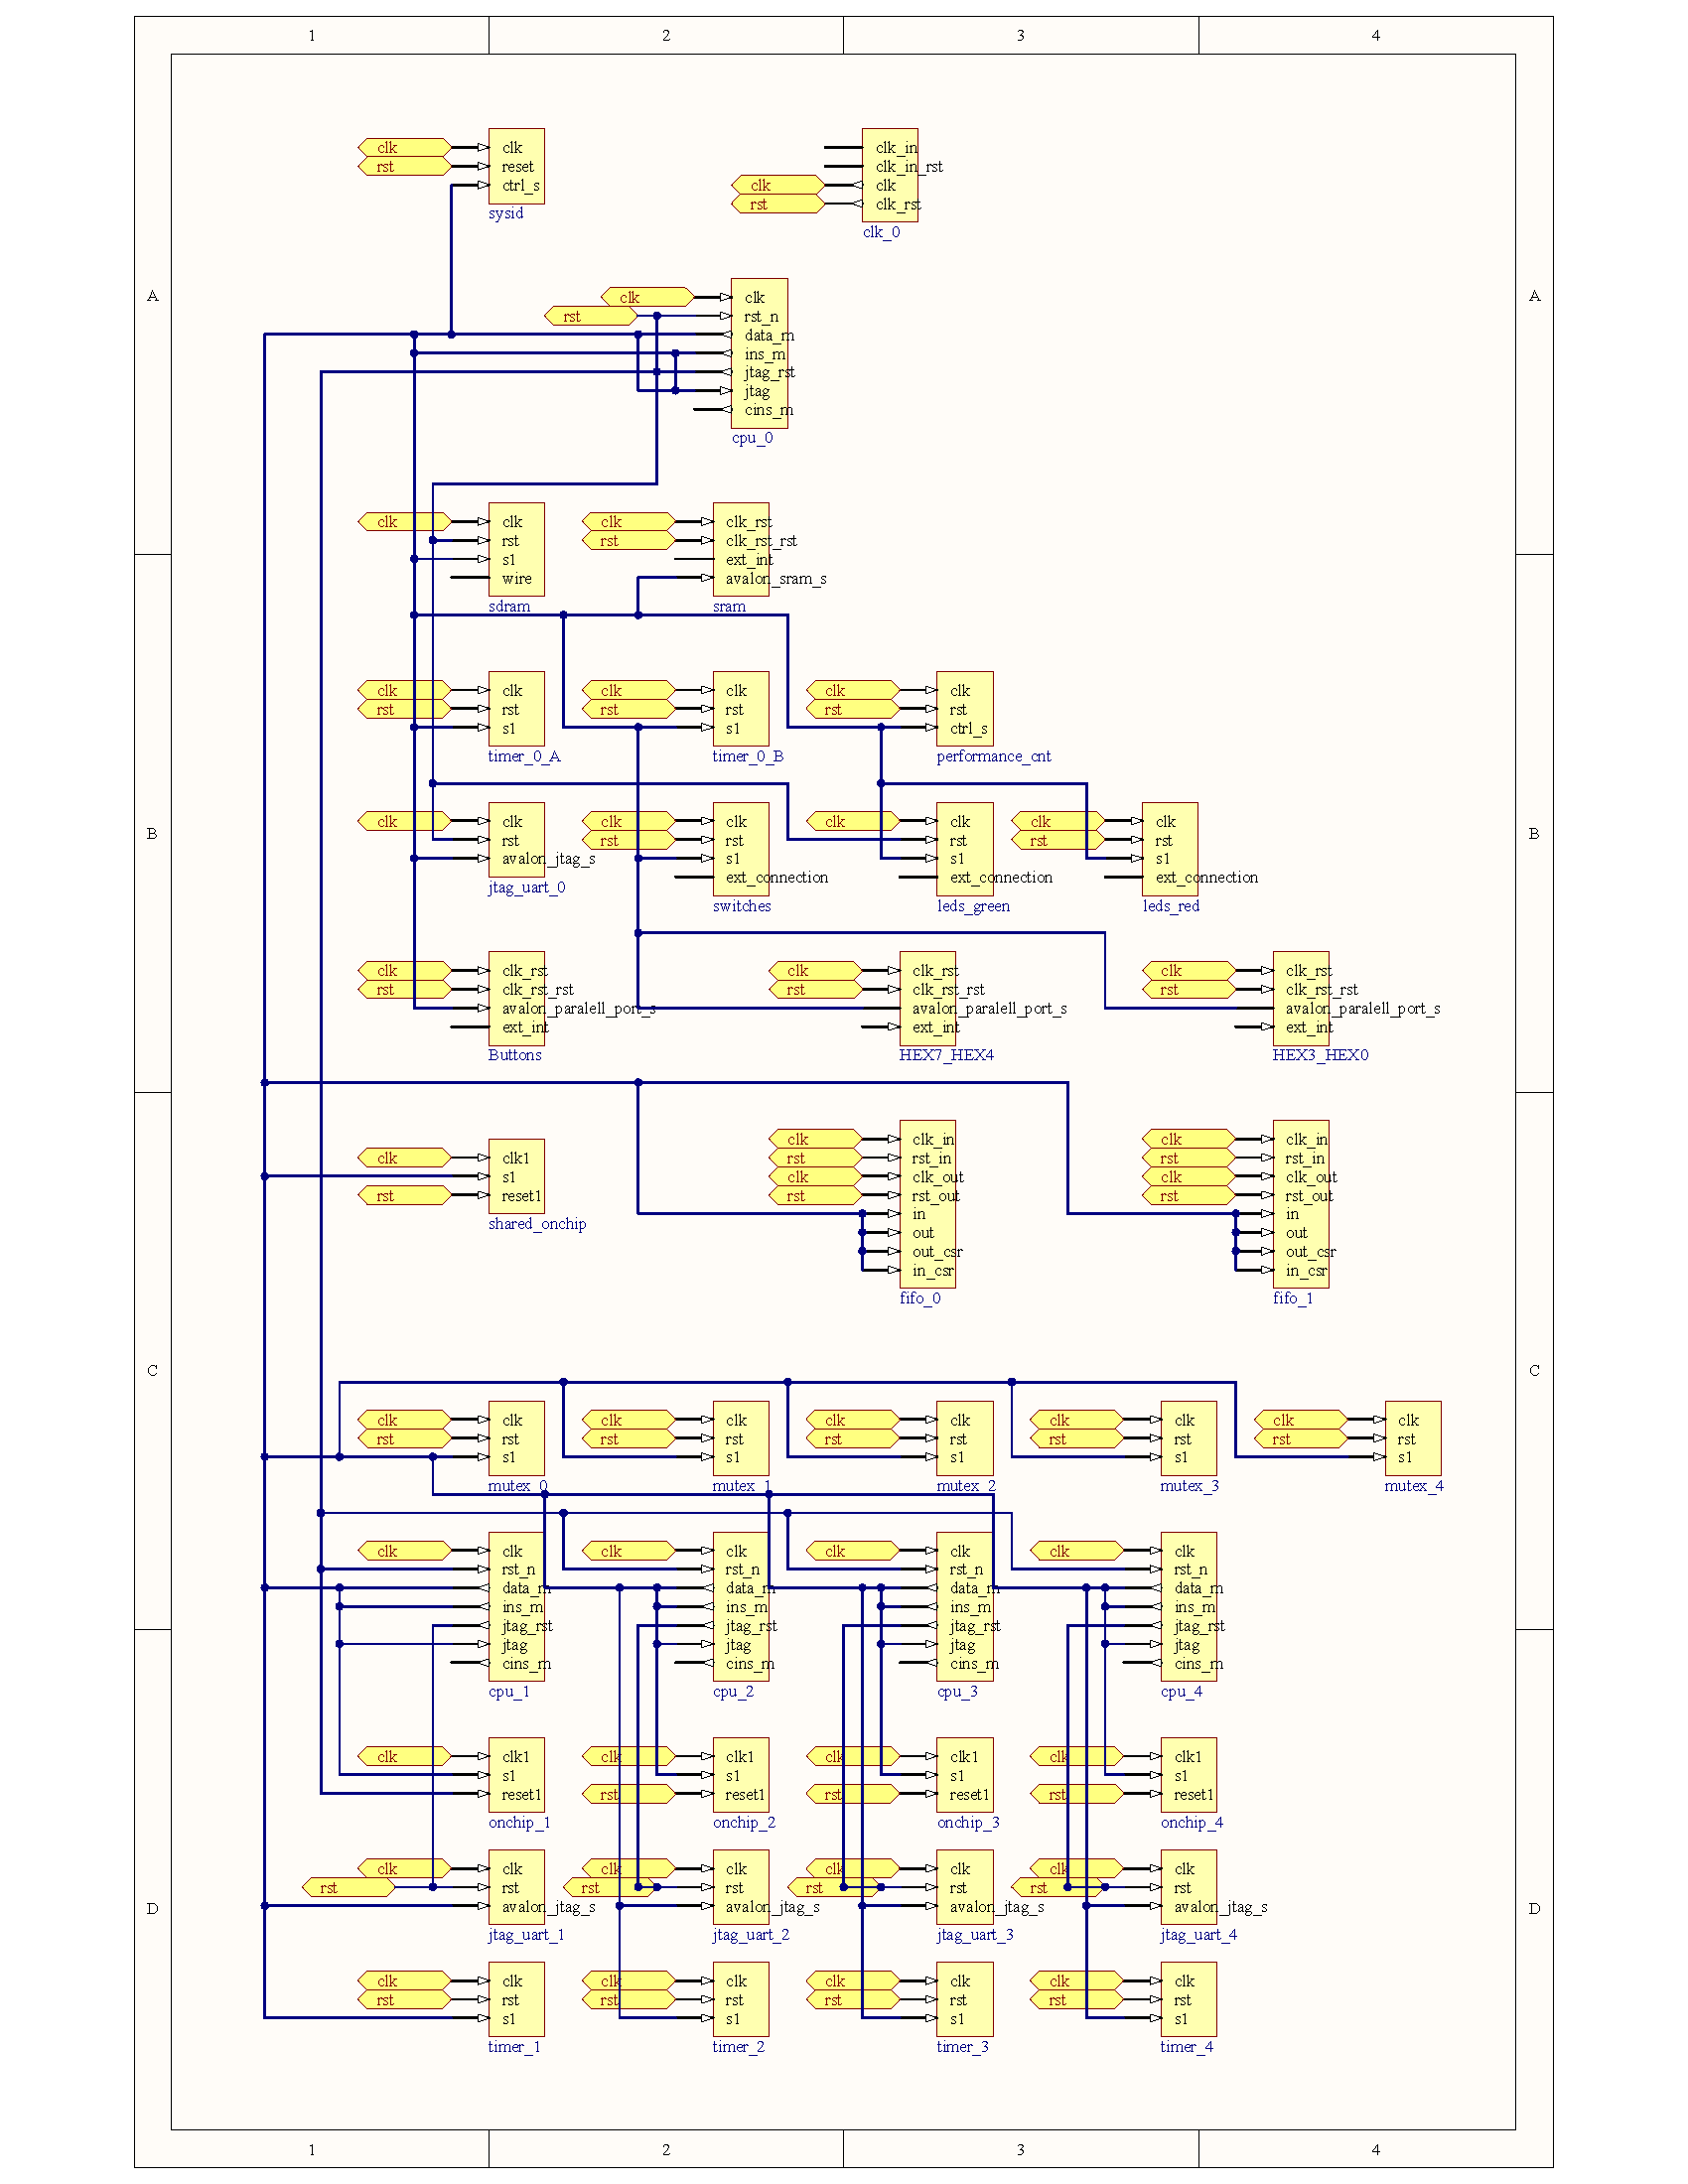
\includegraphics[scale=0.87]{SchematicPrints.png}
%	\caption{Detailed Interconnection Graph}
%	\label{SchematicPrints}
%\end{figure*}





% trigger a \newpage just before the given reference
% number - used to balance the columns on the last page
% adjust value as needed - may need to be readjusted if
% the document is modified later
%\IEEEtriggeratref{8}
% The "triggered" command can be changed if desired:
%\IEEEtriggercmd{\enlargethispage{-5in}}

% references section

% can use a bibliography generated by BibTeX as a .bbl file
% BibTeX documentation can be easily obtained at:
% http://mirror.ctan.org/biblio/bibtex/contrib/doc/
% The IEEEtran BibTeX style support page is at:
% http://www.michaelshell.org/tex/ieeetran/bibtex/
\bibliographystyle{IEEEtran}
% argument is your BibTeX string definitions and bibliography database(s)
\bibliography{bibi}
%
% <OR> manually copy in the resultant .bbl file
% set second argument of \begin to the number of references
% (used to reserve space for the reference number labels box)





% that's all folks
\end{document}



%%% Local Variables:
%%% mode: latex
%%% TeX-master: t
%%% End:
